\documentclass[border=12pt,dvipsnames]{standalone}
\usepackage{pgfplots}
\pgfplotsset{compat=1.17}
\usepackage{xcolor}
\usepackage{amsmath,amssymb}
\usepackage{tikz}
\usetikzlibrary{arrows.meta}

\definecolor{gold}{HTML}{CFB87C}
\definecolor{dkblue}{HTML}{156082}
\definecolor{ltblue}{HTML}{5B9BD5}
\definecolor{dkgreen}{HTML}{196B24}
\definecolor{ltgreen}{HTML}{70B87C}
\definecolor{dkgray}{HTML}{333333}
\definecolor{medgray}{HTML}{888888}

\begin{document}
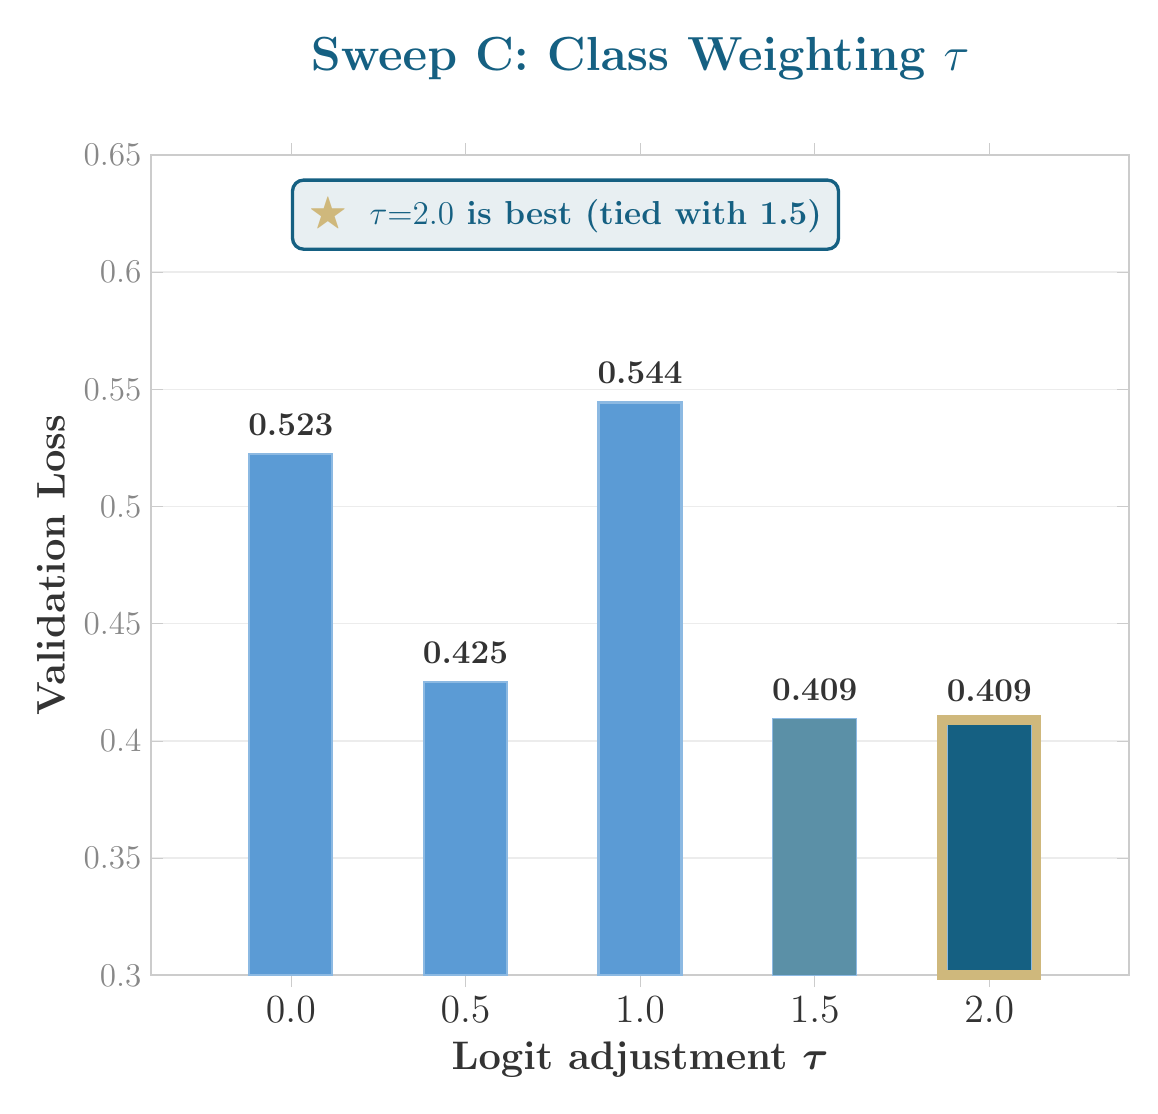
\begin{tikzpicture}
\begin{axis}[
    ybar,
    width=14cm,
    height=12cm,
    bar width=30pt,
    ymin=0.30, ymax=0.65,
    xlabel={\Large\textbf{Logit adjustment~$\boldsymbol{\tau}$}},
    xlabel style={font=\large, color=dkgray},
    ylabel={\Large\textbf{Validation Loss}},
    ylabel style={font=\large, color=dkgray},
    title={\LARGE\bfseries\color{dkblue} Sweep C: Class Weighting $\tau$},
    title style={at={(0.5,1.06)}},
    xtick=data,
    symbolic x coords={0.0, 0.5, 1.0, 1.5, 2.0},
    xticklabel style={font=\Large, color=dkgray},
    yticklabel style={font=\large, color=medgray},
    ymajorgrids=true,
    grid style={gray!15, line width=0.5pt},
    axis line style={gray!40, line width=0.8pt},
    tick style={gray!40},
    nodes near coords,
    every node near coord/.append style={font=\large\bfseries, color=dkgray, anchor=south, yshift=3pt},
    point meta=explicit symbolic,
    clip=false,
    enlarge x limits=0.2,
]

\addplot[
    ybar,
    fill=ltblue, draw=ltblue!70, line width=0.8pt,
] coordinates {
    (0.0, 0.5225) [0.523]
    (0.5, 0.4252) [0.425]
    (1.0, 0.5444) [0.544]
    (1.5, 0.4094) [0.409]
    (2.0, 0.4090) [0.409]
};

% Color overlay for winner bar (tau=2.0)
\fill[dkblue]
    ([xshift=-15pt]{axis cs:2.0, 0.30}) rectangle ([xshift=15pt]{axis cs:2.0, 0.4090});

% Gold border on winner bar
\draw[gold, line width=3.5pt]
    ([xshift=-17pt]{axis cs:2.0, 0.30}) rectangle ([xshift=17pt]{axis cs:2.0, 0.4090});

% Also highlight tau=1.5 (tied)
\fill[dkblue!70]
    ([xshift=-15pt]{axis cs:1.5, 0.30}) rectangle ([xshift=15pt]{axis cs:1.5, 0.4094});

% Winner callout
\node[fill=dkblue!10, draw=dkblue, rounded corners=4pt, line width=1.2pt,
      font=\large\bfseries, text=dkblue, inner sep=6pt,
      anchor=north west]
    at (axis cs:0.0, 0.64) {\raisebox{0pt}{\color{gold}\Large$\bigstar$}\; $\tau{=}2.0$ is best (tied with 1.5)};

\end{axis}
\end{tikzpicture}
\end{document}
